\documentclass[11pt]{IEEEtran}
\usepackage{graphicx}
\usepackage{amsmath}
\usepackage{cite}
\usepackage{booktabs}
\usepackage{hyperref}


\markboth{PV2023: Adding value (to) and preserving Scientific & Technical data, 2-4 May 2023 CERN}{Last Name \MakeLowercase{\textit{et al.}}: Title}

\title{ The Challenge of Digital Preservation at CERN }
\author{Antonio Vivace, Jean-Yves Le Meur\\
    \{antonio.vivace, jean-yves.le.meur\}@cern.ch}
\begin{document}
\maketitle

\begin{abstract}
    This paper outlines the challenge of preserving the vast and diverse amount of digital content generated by the CERN community.

    First, we define the initial scope of preservation, giving an overview of the digital repositories selected for developing an OAIS-compliant archive at CERN.

    The OAIS reference model will then be briefly introduced, explaining the fundamental components of a digital preservation system and how they are being implemented.

    Next, we introduce the CERN Digital Preservation platform, which is designed to orchestrate these components and enable existing information systems to adopt a preservation strategy. We highlight how existing tools and digital preservation solutions, such as Archivematica, are being integrated into this platform.

\end{abstract}

\section{Preservation scope}

Scientific and institutional data produced at CERN is disseminated on a number of different repositories and internal or external content management systems.

Below are listed some of the information systems considered during this initial phase.

\subsection{Institutional Repositories (IRs)}

\textbf{Zenodo} is a general general-purpose open repository hosting research papers, data sets and research software. Targeted at a wider world audience. It is based on the InvenioRDM \cite{InvenioRDMinveniosoftwareorg-2023-03-16} software.

\textbf{CERN Document Server} (CDS) is a repository dedicated to documenting articles, reports, and multimedia content in High Energy Physics (HEP). It includes articles and preprints, books and proceedings, presentations and talks. It is powered by an old version of the Invenio software.

\textbf{Indico} is a powerful event (meetings, conferences, lectures) management system.

\textbf{CERN Open Data portal} is the access point to a growing range of data produced through the research performed at CERN. It disseminates the preserved output from various research activities and includes accompanying software and documentation needed to understand and analyse the data.

\subsection{Other systems}


\textbf{GitLab} is a web-based Git repository and collaborative software development platform that offers code hosting, project management capabilities, wikis, continuous deployment and integration pipelines. A large part of the software developed at CERN experiments and IT projects is hosted on a CERN instance of GitLab.

\textbf{CodiMD} is a platform that allows editing and sharing text documents in Markdown. It is often used to prepare internal drafts or informal documentation.


\section{Implementation}

The OAIS Reference Model\cite{OAIS2002} (ISO 14721) is considered the fundamental standard for digital preservation. It provides requirements and standards for an archive or repository to provide long-term preservation of digital information.

A preliminary inspection was conducted on the mentioned repositories, which are looking for an optimal strategy to digitally preserve their assets. They lack the functionality for creation of the Archival Information Packages (AIPs) that are the main component of OAIS. AIP is defined by OAIS as the final package of information and metadata that is prepared by the archive before being stored for the long-term preservation of the digital object.

Below are explained the developments that were carried out to assist IRs in becoming OAIS compliant.

\subsection{Environment}

A digital preservation strategy\cite{strategy} is proposing three options to move towards OAIS compliance:

\subsubsection{Preservation is performed by the IR} The IR handles preservation actions and a registry internally without using a dedicated central service. A central entity will only ensure that it is implemented following OAIS and may harvest the IR's preservation registry to feed into a central registry.

\subsubsection{Preservation is shared between the IR and the Digital Preservation Service}

The Information Repository is responsible for creating Archival Information Packages in formats aligned with CERN specifications and for performing migrations when required. These AIPs are deposited in a central digital preservation registry maintained by the Preservation service. Versioning and transferring AIPs to the CERN Tape Archive or remote long-term storage for bit preservation is under the responsibility of the preservation service.

\subsubsection{Preservation is delegated to the Digital Preservation service}

The Digital Preservation service supports an “AIP Factory”. It provides IRs with a protocol to push or pull the original content to be preserved according to a Submission Information Package (SIP) specification. Preservation processes are performed according to current standards using existing specialized software (such as Archivematica). The final AIPs are stored on tape and can be retrieved at any time by the submitting IR.

\subsection{CERN SIP Specification}

\begin{figure}
    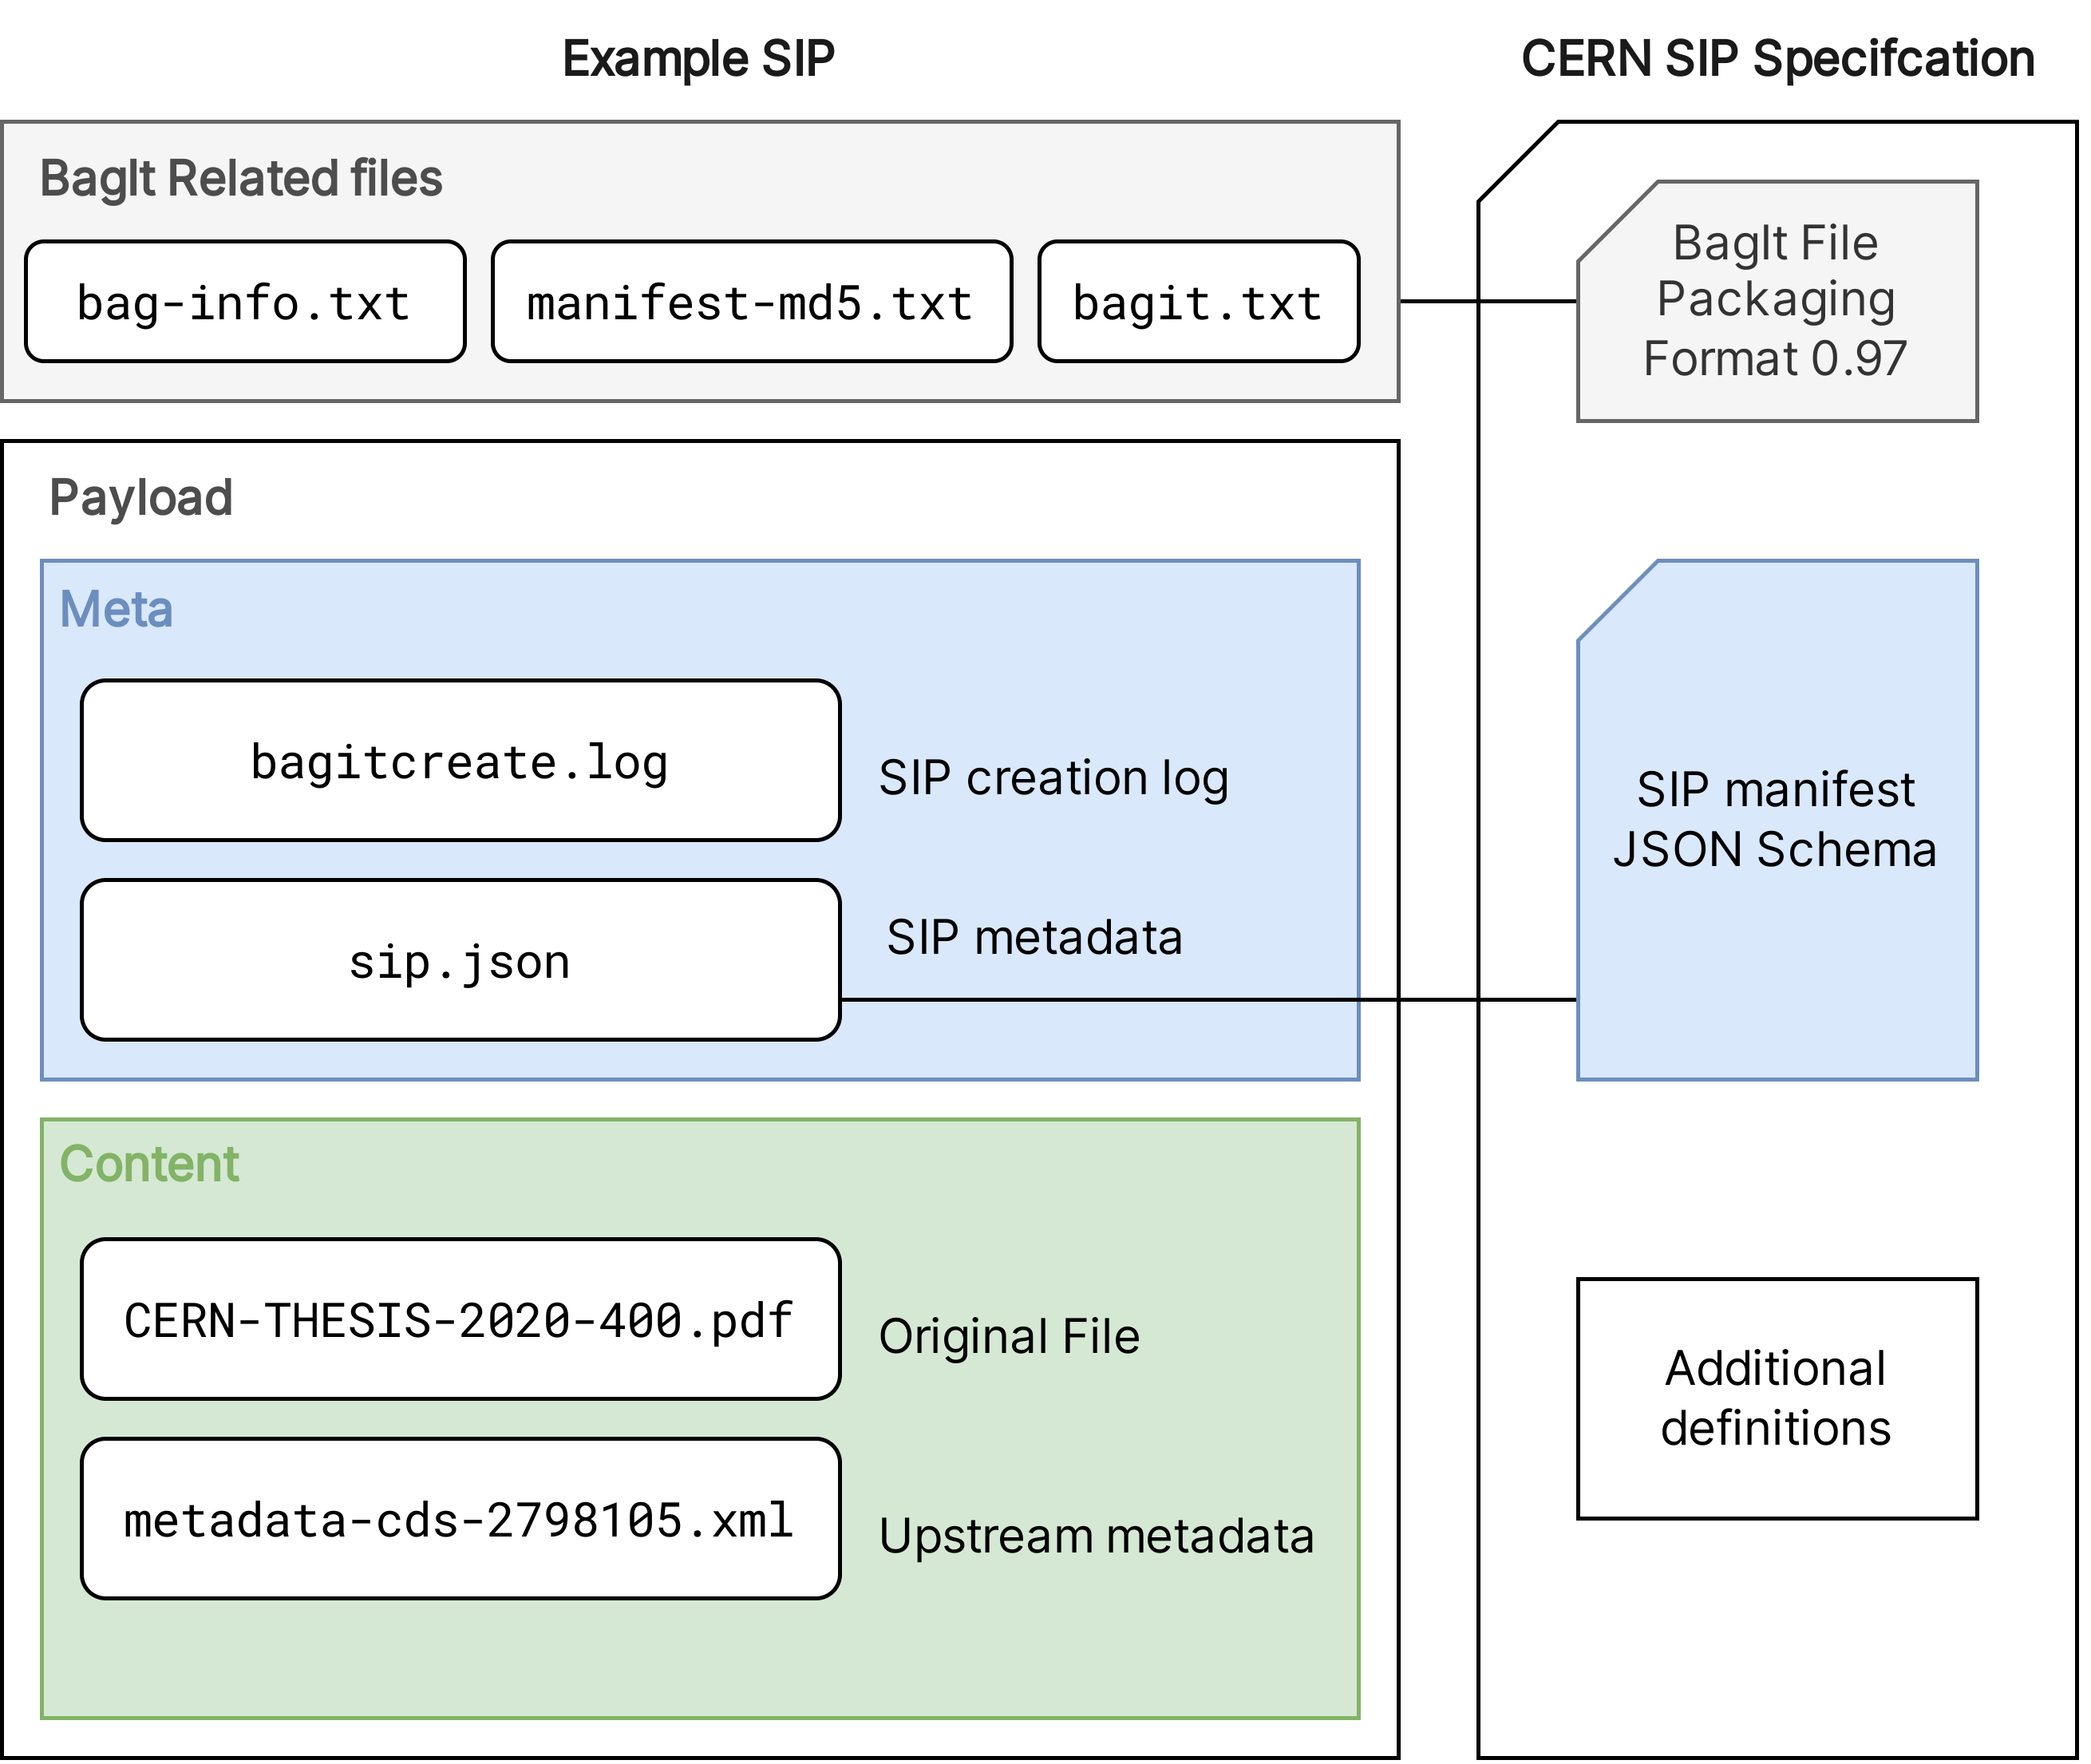
\includegraphics[width=3.5in]{sip_spec.drawio.png}
    \caption{Structure of the CERN SIP specification and an example SIP created from a record on the CERN Document Server.}
\end{figure}

Submission Information Packages (SIP) are defined by the OAIS reference as Information Packages  delivered from the source IRs to the preservation system for ingest. Ingestion, in this model, is the process that verifies the consistency of the content and all its related metadata, computes preservation checksums for all the files and extracts some additional metadata.

Following this standard, we developed a CERN SIP specification \cite{CERNDigitalMemorySIPSpecGitLab-2021-09-15}, mandating how a data record can be packaged, in which form its payload must be stored and how should the required and optional metadata be specified.

The CERN SIP consists of a folder conforming to the BagIt File Packaging Format specification, a popular Internet Draft that defines a file system structure for transferring and archiving a collection of files.

Contents of such bags are provided and organised in accordance with an additional specification, described by the following components:

\begin{enumerate}
    \item A text document, explaining the specification with examples and how the various requirements from the OAIS reference model are implemented.
    \item The JSON Schema of the manifest, where high-level metadata such as provenance is described.
    \item A validation software library in Python, that enables to verify that a folder conforms to the CERN SIP and exposes errors or missing data.
\end{enumerate}

\subsection{BagIt Create}

BagIt Create is a software tool to create export packages from the IRs, complying with the CERN SIP specification. It does so by harvesting data from the upstream sources and using the official exposed APIs (if any). It can be imported into any Python script or used standalone as a command line tool. 

Each source is supported by writing a pipeline implementing specific steps. The tool is very modular; additional pipelines can be easily created to support new repositories or extend existing ones.

BagIt Create also supports local files and folders, allowing users to create SIPs even for data simply lying on disk.

Two example cases in which the tool has already been proven useful are the following:

\par{\textit{Department Head finishing their mandate}}

When the previous CERN IT Department Head finished his mandate, BagIt Create and the platform were used to create SIPs from data that was never published in canonical repositories (e.g. local files, notes, etc.).

\begin{figure*}
    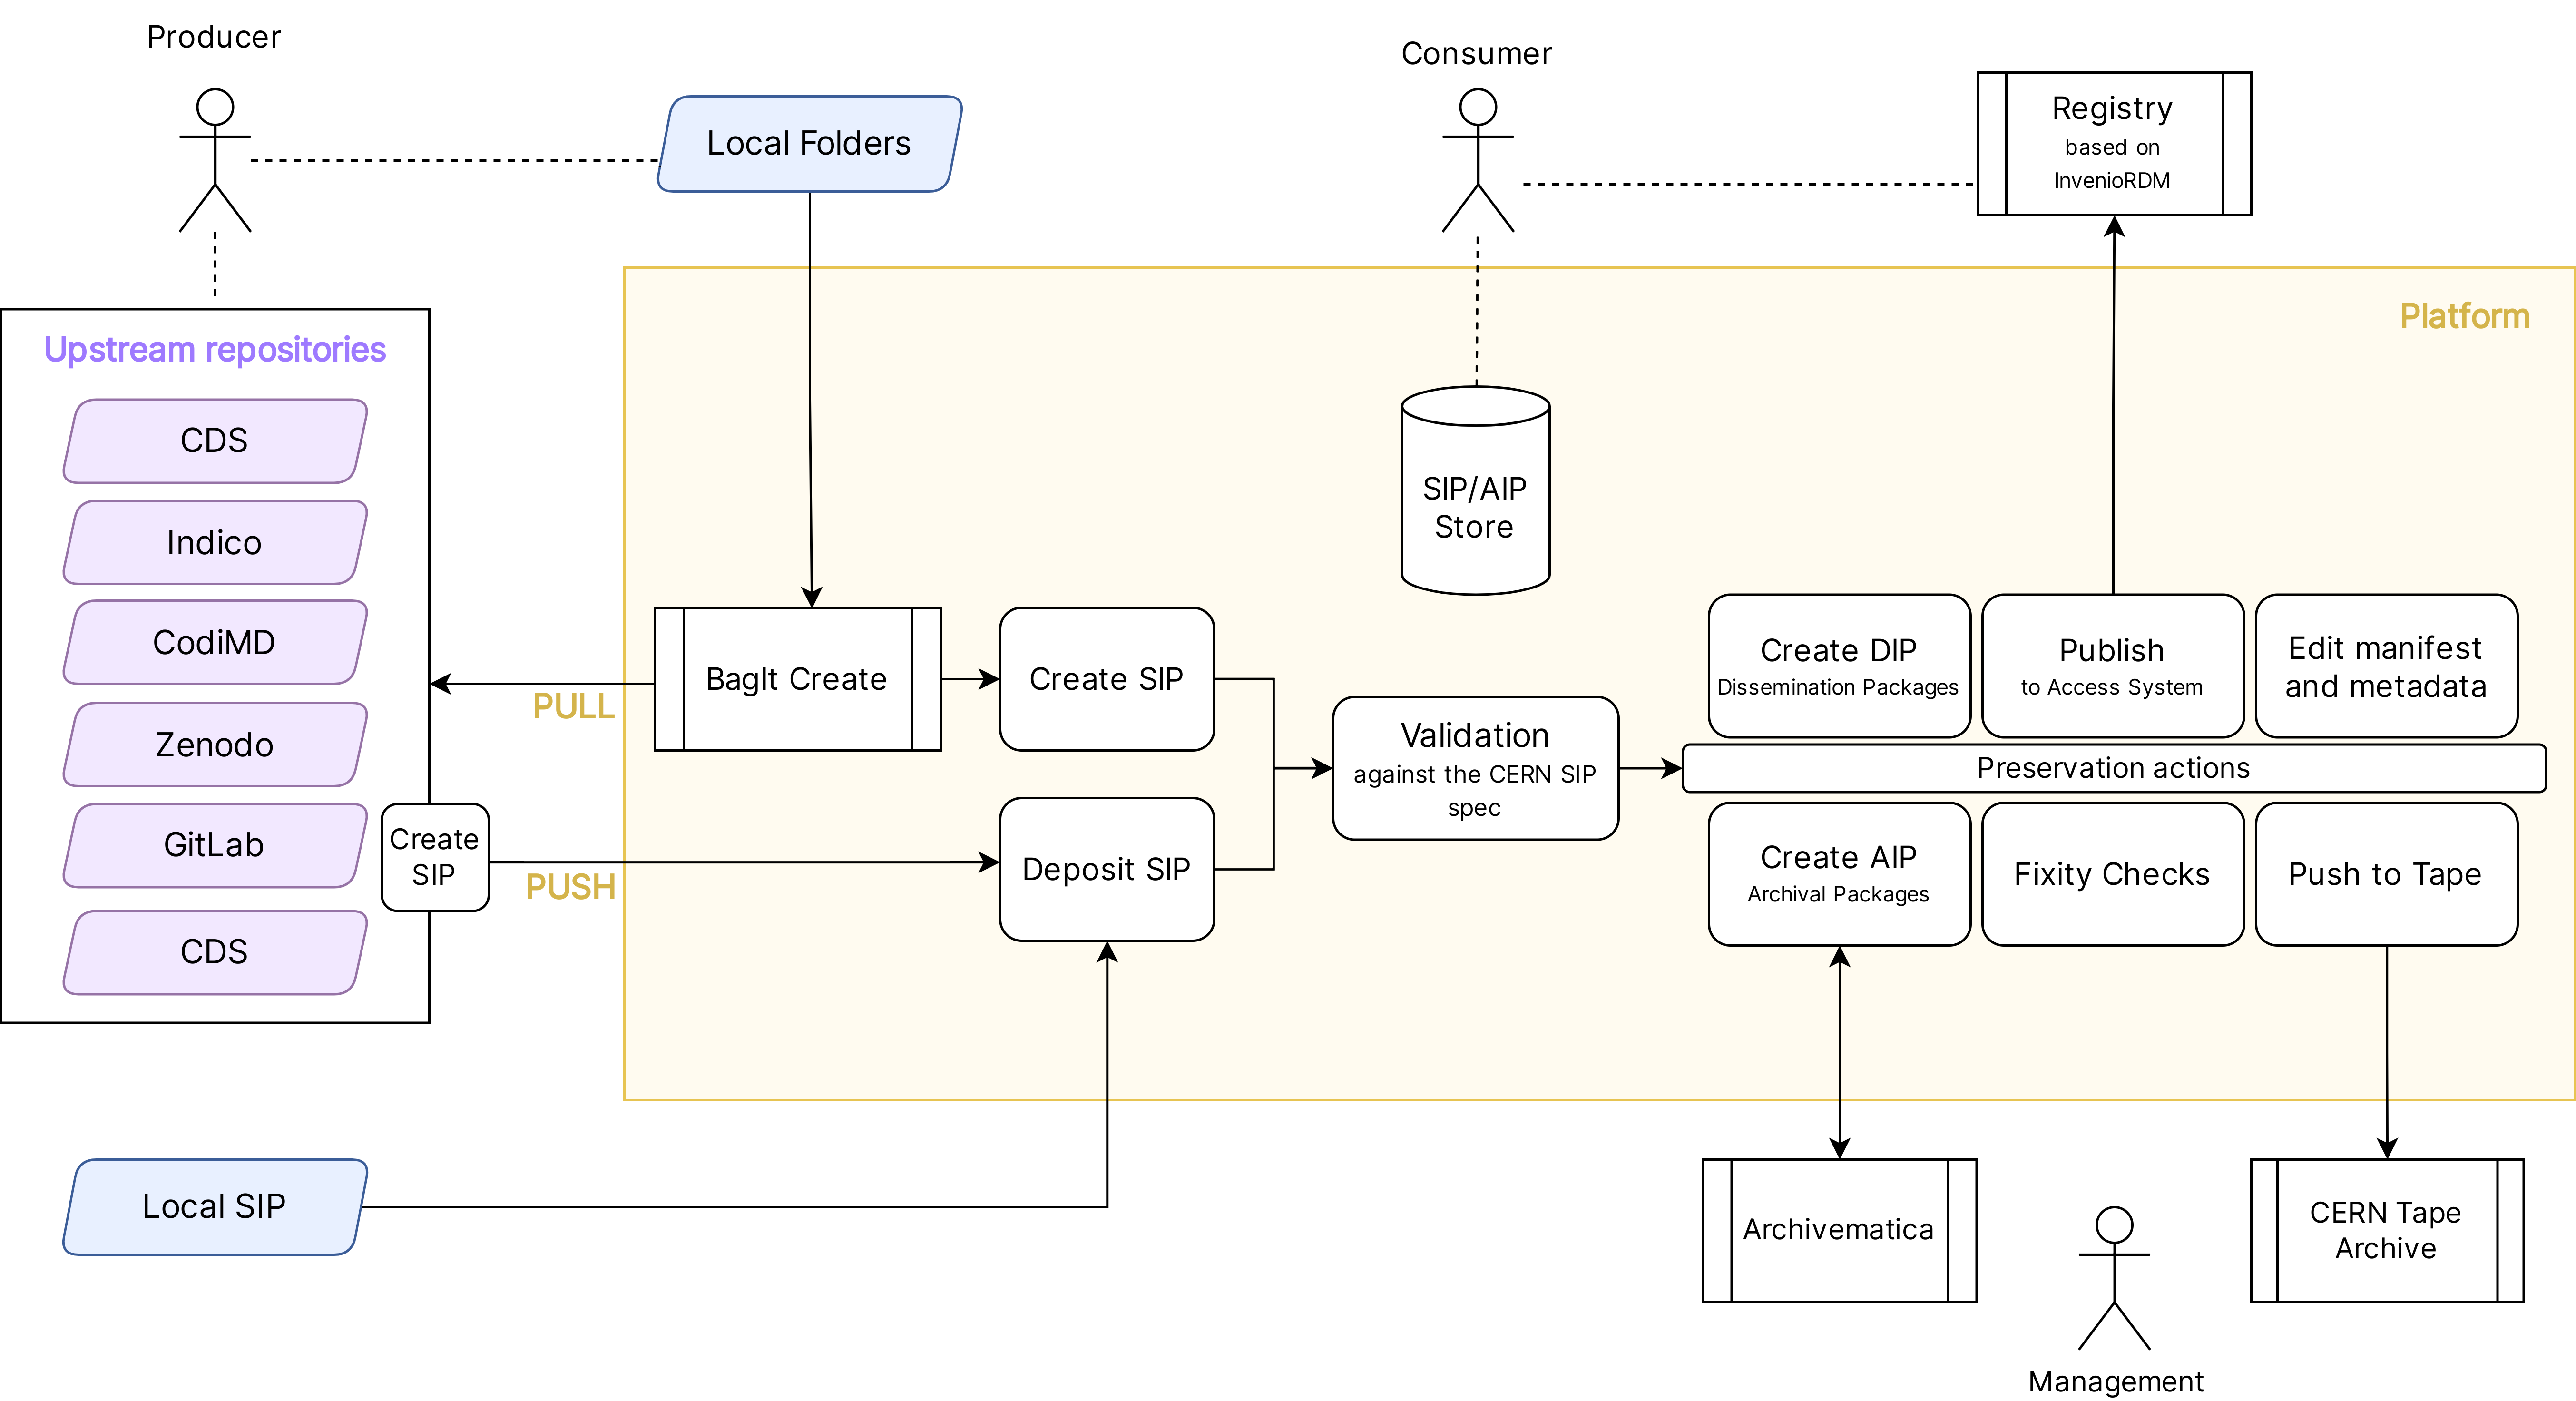
\includegraphics[width=\textwidth]{platform2.drawio.png}
    \caption{Overview of the data flows and components of the Digital Memory platform.}
\end{figure*}

\par{\textit{Decomissioned repository}}

ILCDoc was a document repository based on an old version of Invenio, hosting resources related to the International Linear Collider, a proposed linear particle accelerator. It also had a related Indico instance for events and conferences called ILC Agenda.
ILCDoc was decommissioned in 2022, and the machines running it were put offline.

Before so, we ran an archival operation creating packages for every document in ILCDoc and every event they referenced in the Agenda.


\section{Platform}

The central element of the proposed preservation service is a full-stack application, the Digital Memory platform.

Its primary purpose is to execute and orchestrate preservation tasks, some internally and others interacting with external services and components.

A web interface (in React) or a REST API can be used to interact with the platform.


\subsection{Workflow}


The platform can \textit{harvest} records from the upstream IRs. It uses the BagIt Create tool to \textbf{pull} the data and create SIPs for the records requested by the user of the platform. Records can be retrieved by querying the IRs directly from the platform or by providing links and unique IDs of the records to harvest.

Alternatively, the SIP can be created by the IRs and deposited to the platform (\textbf{push}) using a dedicated deposit API route.
\\

Once the SIP is in the platform, the SIP validation tool is run on the package, verifying integrity and compliance with the CERN SIP specification. If this succeeds, fixity checks are run, and additional checksums may be computed.

At this point, the following steps can be triggered, either by an operator or automatically:

\begin{itemize}
    \item AIP creation. The SIP is sent to Archivematica\footnote{An integrated suite\cite{Archivematica} of open-source software tools to process digital objects for digital preservation in accordance with ISO-OAIS.}. This process includes converting file formats to their preservation (open standards) counterparts \cite{FormatpoliciesArchivematica}, extracting metadata and much more.
    \item Push to Cold Storage. The packages can be queued up and prepared to be pushed to the CERN Tape Archive for the long term.
    \item Publish the archival packages on the Digital Memory Registry. The record and the related assets are published on an access system powered by InvenioRDM. Multiple versions can be published (e.g. referring to the same upstream record but at a different time or to the same data undergoing different preservation actions).
\end{itemize}

\begin{figure}
    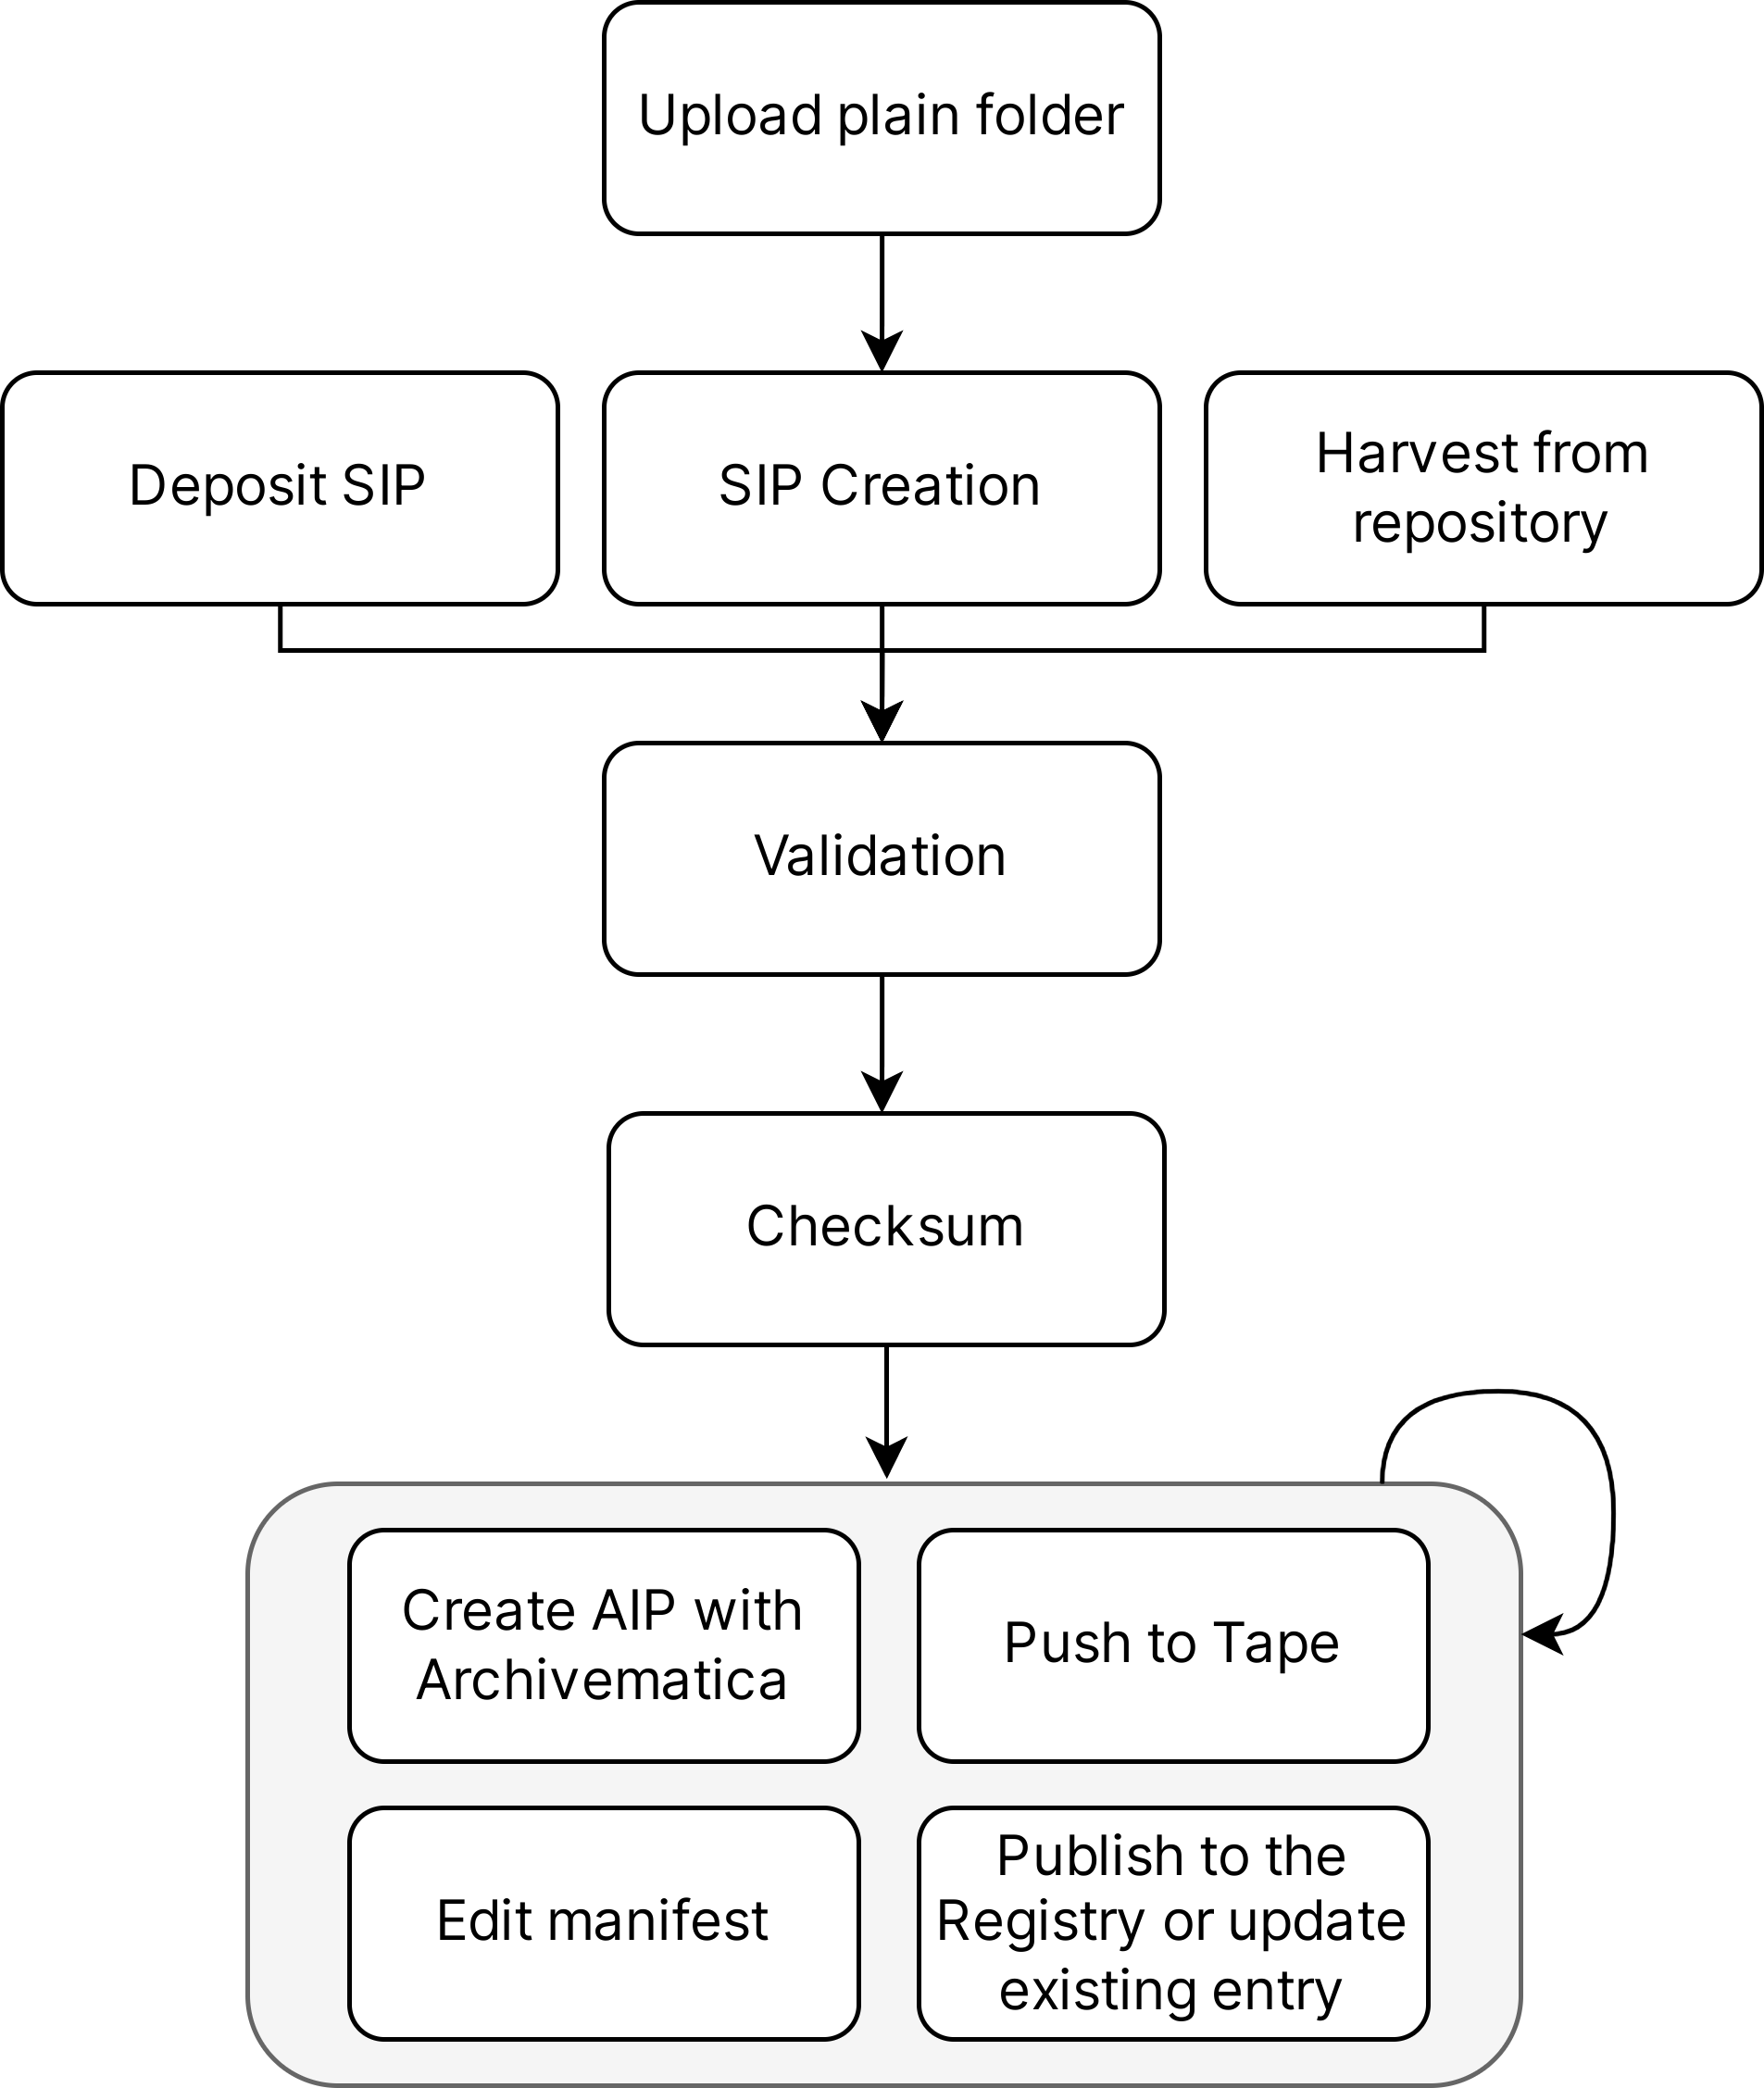
\includegraphics[width=3.4in]{pipeline.drawio.png}
    \caption{Steps in the preservation pipeline.}
\end{figure}

\subsection{User workflow}

We also implemented a \textit{self-service area}, where CERN users can autonomously log in using their credentials (through the CERN SSO) and access the platform. This empowers the user to:

\begin{itemize}
    \item Select what they may want to archive
    \item Add some additional metadata and perform additional curation
    \item Organize what they are archiving by applying "tags"
    \item Let the platform fetch the resources they requested
    \item Download archival packages for their personal usage
    \item Submit assets for long-term preservation
\end{itemize}

This aims to cover the cases of users leaving CERN, changing projects or experiments, changing their contracts or simply wanting to do a periodic review of what they produced.

\subsection{Technology}

Every component of the Digital Memory platform is released as Open Source software \cite{CERNDigitalMemoryGitLab-2023-03-01}, and it’s designed to be reusable and adaptable to more generic setups.

\subsubsection{Django}

The backend was built upon Django and the Django REST Framework. All the functionalities are exposed by a RESTFul API, which is documented by an OpenAPI 3 specification. Asynchronous executions of more demanding tasks are carried out by Celery workers.

\subsubsection{Archivematica Helm Charts}

To minimize maintenance and downtime, we decided to deploy Archivematica and all the required infrastructure on a Kubernetes cluster.

The deployment was made reproducible and scalable by building Docker images of the Archivematica dependencies and preparing Helm charts \cite{archivematicak8s} to bring up the whole stack.

Although some CERN specifics settings are used (because we deploy on the CERN OpenShift service and we use CERN-specific storage), the charts are easily adaptable to be deployed on other Kubernetes clusters.

\subsubsection{Deployment}

Docker images of the platform are automatically built on the CI/CD pipeline. They include a complete and reproducible environment for the backend and the frontend stack.

Helm Charts are provided here too to ease the deployment on Kubernetes-based solutions (such as OpenShift).

Integration and deployment pipelines were developed and hooked to the git repositories, so test instances could easily follow code changes.

Detailed documentation guides the operator through the deployment process and the configuration of all the connected components (e.g. InvenioRDM, EOS storage, CERN Tape Archive, CERN SSO, Sentry diagnostics, ..).

\section{Conclusion}

Possible further improvements include:

\subsection{Moving SIP creation to the repositories}
The current approach of delegating to BagIt Create the export functionality is tied to the stability of the various API surfaces it consumes. Even if it currently works, it would be unrealistic to have a central piece of software that has to maintain compatibility with several different ever-changing IR software and the API they expose. A more sustainable solution may pass by delegating the responsibility of these "connectors" to the maintainers of the IR or directly moving these implementations to the codebase of the IR, so they can adequately export complying SIPs.

\subsection{Appraisal and content selection}

IRs and organisation-level policies should be adopted to define which kind of content should receive which type of preservation treatment.

E.g. a specific category of institutional events may require multiple copies on tape and be disseminated publicly from the registry. In contrast, ex-employee personal documents may not require preservation versions but be available to the teams currently working on those projects.


\subsection{Archivematica and the support for Office documents}
Archivematica does not currently support Microsoft Office documents; preservation versions of those files are not prepared during the AIP creation process.
The Archivematica team is surveying which tools should be officially adopted to complete this task. Still, an alternative should be found for the time being since Office documents make up for a considerable amount.

\subsection{Access to the Registry}
At the moment, the Digital Memory registry is accessible only to administrators.

Although the distribution of public content may be unrestricted, IRs must agree upon and adopt policies governing access to private and protected data in the registry.

An initial proposal may be based on the current rules of the paper archives \cite{CERNArchiveAccessRules}.


\bibliographystyle{IEEEtran}
\bibliography{references}


\end{document}
